\chapter{Results and Discussion}

\section{Performance analysis}

To determine the effects of different cluster configurations on the achievable system performance, analysis needs to be conducted 

\subsection{Key metrics}

There are three key metrics that will be used to assess system performance impacts: the HTTP response time, throughput, and error rate. Within the context of self-adaptive systems, as described by \citeauthor{weyns_engineering_2018} \cite{weyns_engineering_2018}, there are two levels of a system that can be optimised. Improvements can be made to the inner managed system, or to the outer managing system. For the Ahuora Digital Platform, the optimisation explored here will focus on optimisation of the managing system, or the Kubernetes cluster. These metrics will serve to inform steps towards such optimisation.

\subsubsection{Response time}

The response time for an individual request is the total length of time taken to receive a response from a destination endpoint. This includes the duration of all steps involved in the request, including the time taken to establish an initial connection, perform a TLS handshake, wait for the response, and receive the data. As a metric, it allows an analyst to observe how a system responds over time to increasing load, with a worsening response time indicating that the system is being throttled or is reaching a performance ceiling. From a developer perspective, the response time is important to track, as an increasing response time worsens the experience for users of a product, who may perceive a slowly responding application as a reflection of poor software quality.

\subsubsection{Throughput}

The throughput of a system is the number of requests that are processed per second. This metric can be used to identify the peak capacity of the system, as well as identify the thresholds or points at which system performance degrades. As opposed to the response time, which is concerned with the performance of individual requests, throughput is a metric that provides insight only with respect to behaviour of the overall system. One goal within a performance optimisation context is to maximise the peak throughput of a system to serve more users concurrently.

\subsection{Secondary metrics}

\subsubsection{Error rate}

Along with speed-oriented metrics like the response time and throughput, it is critical to keep track of the error rate, or the proportion of HTTP requests that failed. Error rates can increase under overloaded system conditions, and can provide early indication that a sustainable throughput threshold has been passed. Another reason to record errors is to prevent invalid observations being made about test results. In some situations, failed requests may have lower response times than their successful counterparts, which may mislead one to think the system is more responsive than it actually is.

\subsubsection{Container-level resource utilisation}

Both CPU and memory usage will provide additional insight into system performance influences. For example, the observation of high consumption of allocated CPU time within a pod or container at the same time as observed request rate instability would possibly indicate the pod is reaching computation limits.

\subsubsection{Cluster-level resource allocation and utilisation}

Especially when auto-scaling policies are in place, it is necessary to track the number of deployed pods for each active cluster deployment. This metric can then be used to calculate the sum of all provisioned resources on the cluster, such as the total requested CPU. With this information, the level of over or under-provisioning can be compared across different workloads, and across workload configuration variations. If a pod requests 2000 millicores of CPU, but only uses 100 millicores on average, then this is a clear sign of severe over-provisioning. Likewise, requesting 500 millicores but quickly reaching an average of 90\% CPU utilisation would indicate under-provisioning. With auto-scaling policies in place, poorly set CPU or memory requests can rapidly multiply into cluster-wide resource allocation issues, such as additional pods being unschedulable.

\subsection{Summary statistics}

Using the data generated within tests, a number of summary statistics for each test result can be derived to assist with immediate comparison of deployment configurations.

\begin{itemize}[itemsep=0pt]
    \item \textbf{Average (mean) request completion rate}: The mean number of requests that were successfully completed per second.
    \item \textbf{Maximum request completion rate}: The peak request completion rate across the test duration.
    \item \textbf{Maximum request start rate}: The peak number of requests started by the k6 test client per second.
    \item \textbf{Average (median) response time}: The median time taken for a request to receive a response.
    \item \textbf{Overall error rate}: The proportion of requests across the test that failed due to an HTTP error or client timeout.
    \item \textbf{Performance degradation threshold}: The point at which the response time exceeds a certain level (100 milliseconds for UOR tests, and 1000 milliseconds for FS tests). This statistic allows for an approximation of the request start and completion rates where system performance begins to degrade rapidly. This threshold will not be calculated for average load or stress load tests.
    \item \textbf{Maximum started and completed request ratio}: The largest ratio between the number of requests that have started and the number that have completed. A high ratio indicates that the system is failing to process as many requests as it is receiving. This will not be calculated for breakpoint load tests.
    \item \textbf{Maximum cluster CPU request proportion}: The peak proportion of available cluster CPU used by a deployment. This will be calculated for the Django and IDAES pods only, and only for the resource allocation and utilisation tests.
\end{itemize}

\subsection{Rolling window statistics}

Response times and request rates will be assessed using an exponentially-weighted moving average (EWMA), with a window of ten seconds. Use of a rolling median would appear either too unstable with a small window, or lag behind in showing recent trends. Using an EWMA allows recent data to be paid more attention, and enables better correlation analysis to be conducted.

\section{Unit operation retrieval (UOR) experiment results}

\subsection{Benchmarks}

\begin{figure}[h]
    \centering
    \begin{minipage}{.47\textwidth}
        \centering
        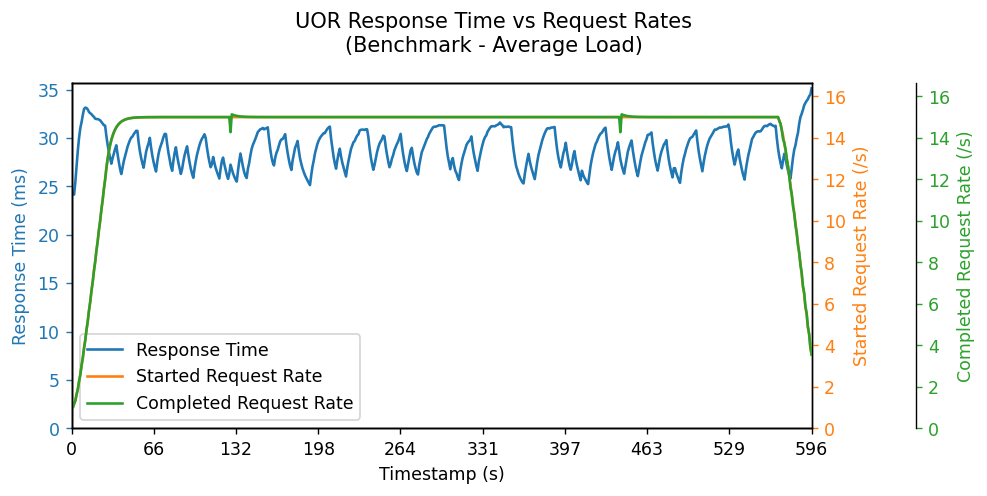
\includegraphics[width=\linewidth]{figures/uor-benchmark-average.png}
        \caption{UOR response time vs. request rate graph - average load benchmark}
        \label{figure:uor-benchmark-average}
    \end{minipage}%
    \hspace{0.05\textwidth} % Adjust the horizontal space here
    \begin{minipage}{.47\textwidth}
        \centering
        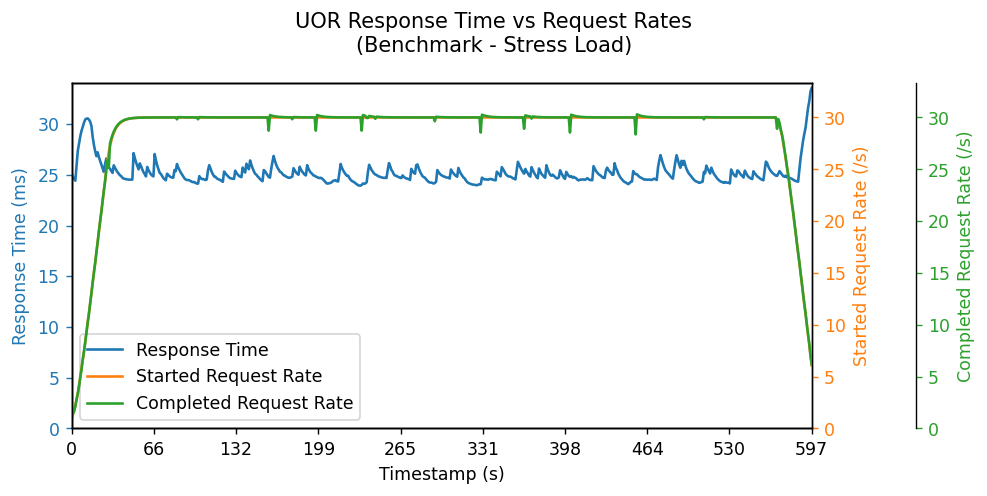
\includegraphics[width=\linewidth]{figures/uor-benchmark-stress.png}
        \caption{UOR response time vs. request rate graph - stress load benchmark}
        \label{figure:uor-benchmark-stress}
    \end{minipage}
\end{figure}

Both response time and request rate degradation can be observed in the local spike test (Fig. \ref{figure:uor-benchmark-spike}). After reaching \textasciitilde40 requests per second, the response time rapidly increases, and the request completion rate starts to diverge from the request start rate. At 45 requests per second (RPS), the response time average increases past 100 milliseconds, and reaches tens of thousands of milliseconds as the request rate continues to increase. During the test, the request start rate is also seen degrading (between 135 and 189 seconds). This is because of the virtual user limit of 2000 set on the k6 test client, which was configured to prevent system resource starvation by the test client. The response time does not appear to recover towards the end of the test. Approximately 0.036\% of requests in the spike tests failed, while neither the average nor stress load tests had any failed requests.

\begin{figure}[h]
    \centering
    \begin{minipage}{.47\textwidth}
        \centering
        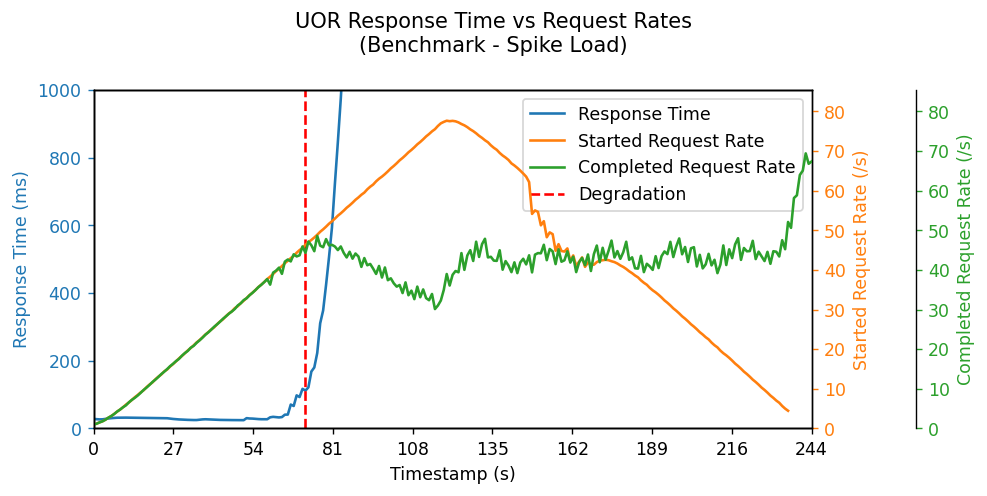
\includegraphics[width=\linewidth]{figures/uor-benchmark-spike.png}
        \caption{UOR response time vs. request rate graph - spike load benchmark}
        \label{figure:uor-benchmark-spike}
    \end{minipage}%
    \hspace{0.05\textwidth} % Adjust the horizontal space here
    \begin{minipage}{.47\textwidth}
        \centering
        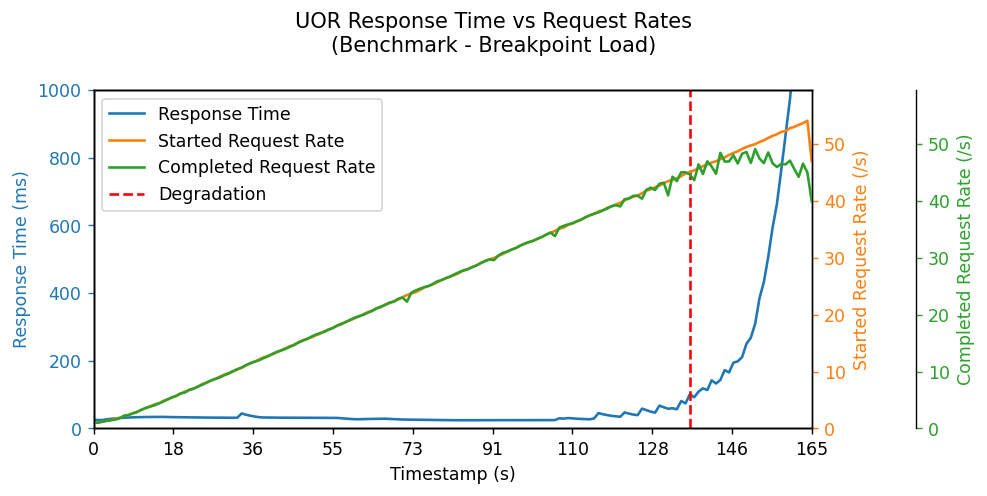
\includegraphics[width=\linewidth]{figures/uor-benchmark-breakpoint.png}
        \caption{UOR response time vs. request rate graph - breakpoint load benchmark}
        \label{figure:uor-benchmark-breakpoint}
    \end{minipage}
\end{figure}

The breakpoint test (Fig. \ref{figure:uor-benchmark-breakpoint}) also identifies this same 45 RPS threshold, beyond which the average response time exceeds 100 milliseconds, and the request completion rate also diverges. No requests failed in the breakpoint tests, but this in part due to the early termination threshold used by breakpoint tests.

\subsection{Replica count}
\label{subsection:fs-replica-count}

\begin{figure}[h]
    \centering
    \begin{minipage}{.47\textwidth}
        \centering
        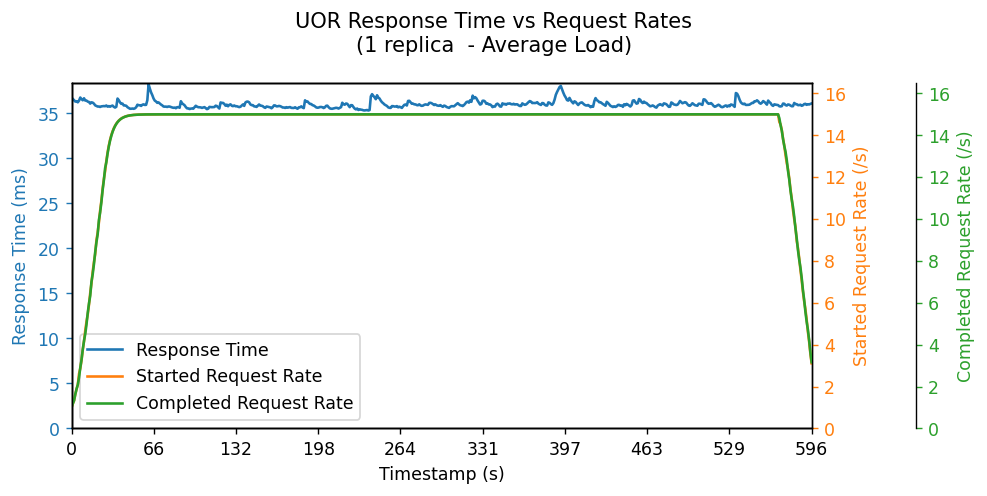
\includegraphics[width=\linewidth]{figures/uor-replica-count-i1-average.png}
        \caption{UOR response time vs. request rate graph - average load with one replica}
        \label{figure:uor-replica-count-i1-average}
    \end{minipage}%
    \hspace{0.05\textwidth} % Adjust the horizontal space here
    \begin{minipage}{.47\textwidth}
        \centering
        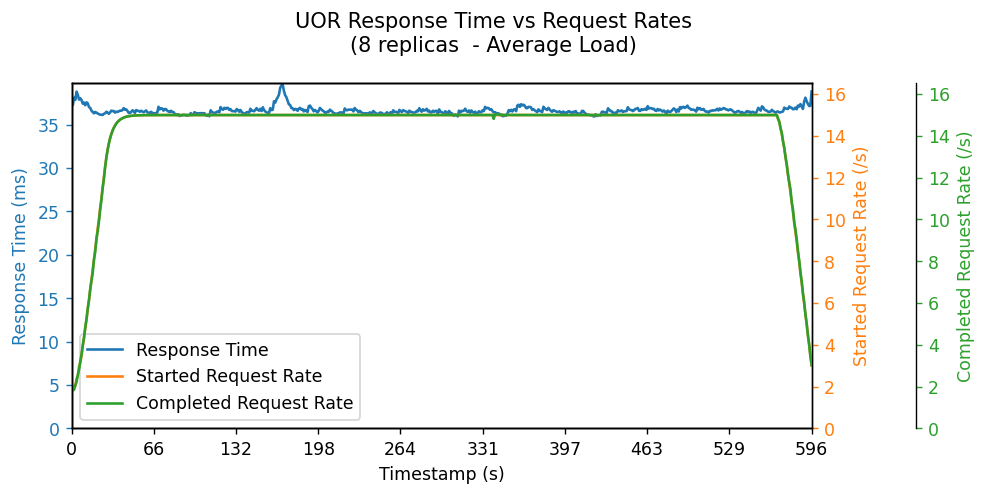
\includegraphics[width=\linewidth]{figures/uor-replica-count-i4-average.png}
        \caption{UOR response time vs. request rate graph - average load with eight replicas}
        \label{figure:uor-replica-count-i4-average}
    \end{minipage}
\end{figure}

\begin{figure}[h]
    
\end{figure}

Using an average load profile against a Django deployment configuration with one replica allows some differences to be observed between the average load benchmark and this cluster-bound test. While the response time of the benchmark sits between 25 and 30 milliseconds, the single replica test sees a median average response time of 35.74 milliseconds (Fig. \ref{figure:uor-replica-count-i1-average}).

\begin{figure}[h]
    \captionsetup{labelformat=empty}
    \caption{Table 1: Table of UOR median response times by replica count, average load}
    \centering
    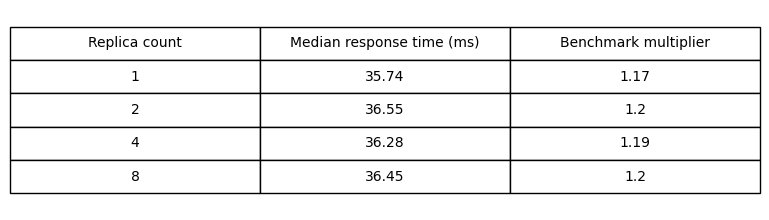
\includegraphics[width=0.8\textwidth]{figures/uor-replica-count-rt-comparison.png}
    \label{figure:uor-replica-count-rt-comparison}
\end{figure}

This higher response time average is consistent with any number of replicas (as seen in Fig. \ref{figure:uor-replica-count-rt-comparison}) when average load is applied. The simple explanation for this difference is the use of TLS in the HTTPS connections used between the test client and the cluster, which may take between 5 and 10 milliseconds per request. Unencrypted HTTP is used to access the local deployment, so less work is required to establish a connection. As well as this, the 5 millisecond artificial delay added for cluster-bound requests partially accounts for this discrepancy. A similar range of averages is observed within the replica count stress tests, albeit with a larger gap between the benchmark and replica count median response times (due to the lower average achieved by the benchmark in stress tests compared with the average load tests.)

Regardless, any tested number of Django replicas running on the cluster is able to process incoming requests as fast as they arrive (evidenced in Fig \ref{figure:uor-replica-count-i1-average} and \ref{figure:uor-replica-count-i4-average}), so there are no significant request rate differences between the benchmarks and the replica count experiments. However, where the benchmarked local deployment shows evidence of performing worse than the clustered deployment is when testing spike and breakpoint loads with more than one replica. As shown in Fig. \ref{figure:uor-replica-count-rt-comp-spike}, a replica count of one performs similar to the benchmark, where the median response time reaches almost 17,000 milliseconds. The median response times for the remaining replica counts (2, 4 and 8) are magnitudes lower, ranging from 39.89 to 42.14 milliseconds.

\begin{figure}[h]
    \centering
    \begin{subfigure}{.5\textwidth}
      \centering
      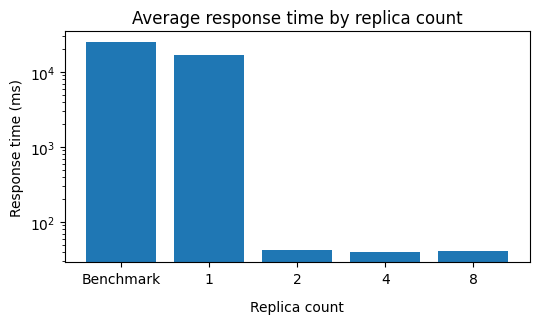
\includegraphics[width=\linewidth]{figures/uor-replica-count-rt-comp-spike1.png}
      \caption{Logarithmic scale}
    \end{subfigure}%
    \begin{subfigure}{.5\textwidth}
      \centering
      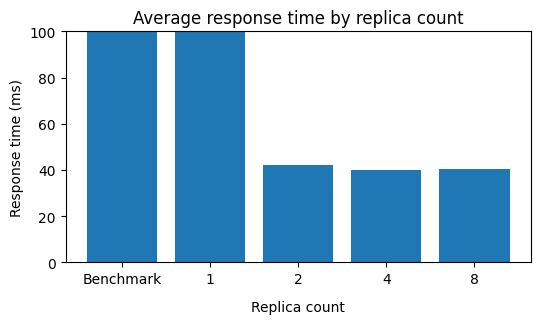
\includegraphics[width=\linewidth]{figures/uor-replica-count-rt-comp-spike2.png}
      \caption{Linear scale}
    \end{subfigure}

    \caption{Median response times by replica count (spike load)}
    \label{figure:uor-replica-count-rt-comp-spike}
\end{figure}

With either four or eight Django replicas, the average response time increases by almost 30\% at the peak request arrival rate (Fig. \ref{figure:uor-replica-count-graph}), but the system is otherwise able to process these requests at the arrival rate. Early signs of degradation are seen when using two replicas, with the response time sharply doubling at the peak request rate, though both request rate curves are mostly consistent \ref{figure:uor-replica-count-graph2}. Interestingly, the response time curve dampening effect with four replicas is highly similar to that with eight replicas, despite doubling the number of available workers. With one replica, this is not the case, having a similar request completion curve (Fig. \ref{figure:uor-replica-count-graph2}) to the benchmark (Fig. \ref{figure:uor-benchmark-spike}), along with an 8.79\% request fail rate, which is 246.35 times worse than the benchmark. The usage of one replica results in the same degradation request rate as the benchmark. None of the other replica count variants have a degradation request rate. When it comes to the started and completed request ratio, a single replica sees a maximum ratio of 1.34 started requests to completed requests, whereas the other replica counts all reach no more than 1.02.

\begin{figure}[H]
    \centering
    \begin{subfigure}{.5\textwidth}
      \centering
      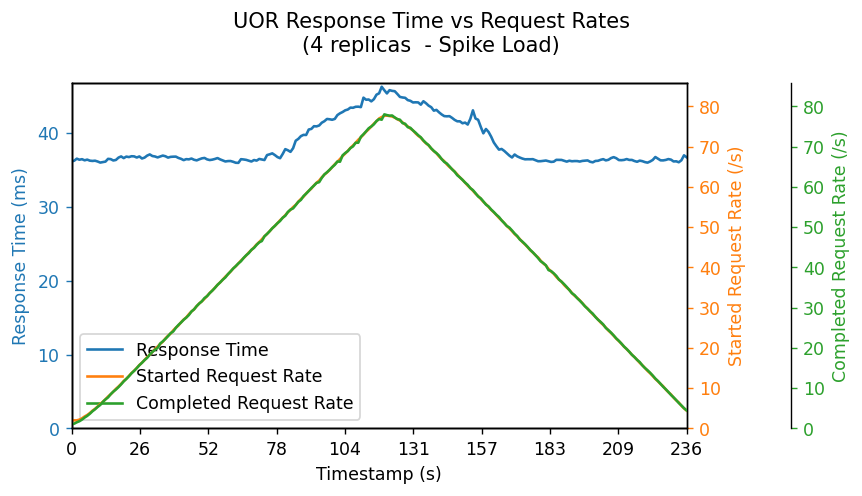
\includegraphics[width=\linewidth]{figures/uor-replica-count-i3-graph.png}
      \caption{4 replicas}
    \end{subfigure}%
    \begin{subfigure}{.5\textwidth}
      \centering
      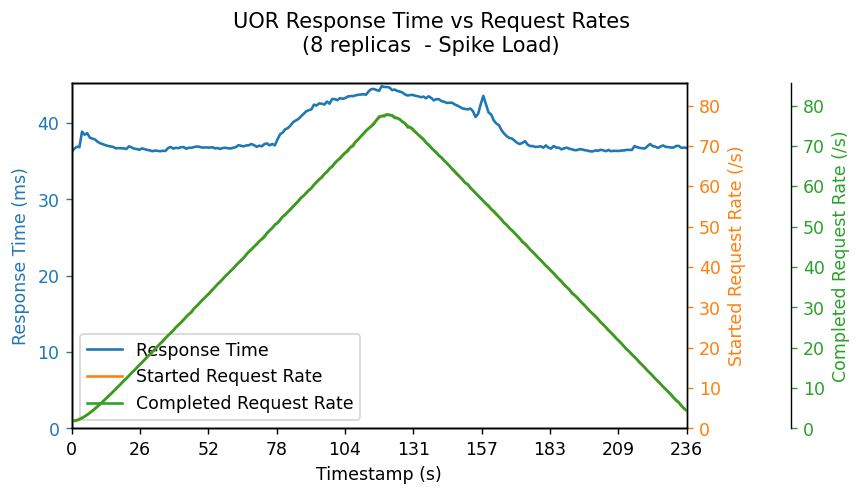
\includegraphics[width=\linewidth]{figures/uor-replica-count-i4-graph.png}
      \caption{8 replicas}
    \end{subfigure}

    \caption{Response time vs. request rate graph (spike load, 4 and 8 replicas)}
    \label{figure:uor-replica-count-graph}
\end{figure}

\begin{figure}[h]
    \centering
    \begin{subfigure}{.5\textwidth}
      \centering
      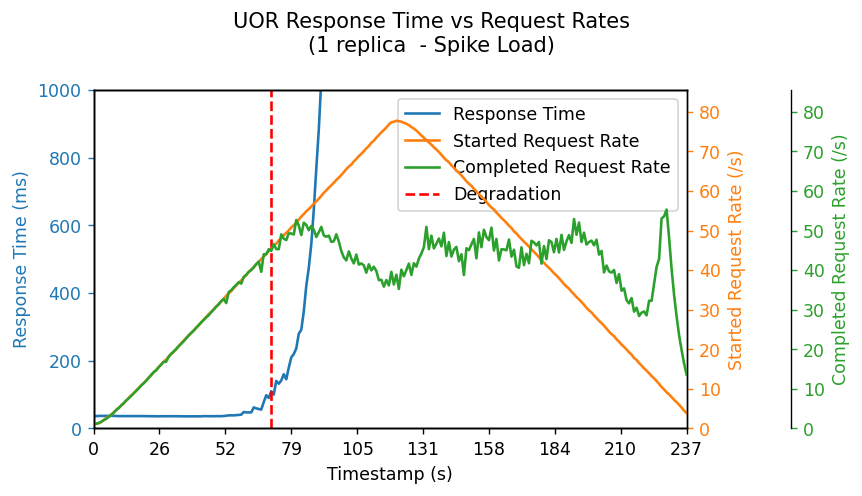
\includegraphics[width=\linewidth]{figures/uor-replica-count-i1-graph.png}
      \caption{1 replica}
    \end{subfigure}%
    \begin{subfigure}{.5\textwidth}
      \centering
      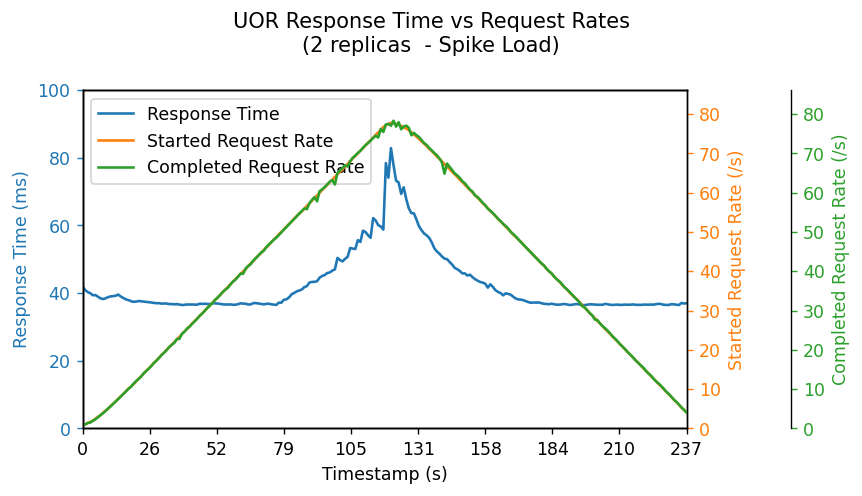
\includegraphics[width=\linewidth]{figures/uor-replica-count-i2-graph.png}
      \caption{2 replicas}
    \end{subfigure}

    \caption{Response time vs. request rate graph (spike load, 1 and 2 replicas)}
    \label{figure:uor-replica-count-graph2}
\end{figure}

Within the breakpoint tests, there is a significant distinction between the maximum request start rate reached across the lowest and highest number of replicas. As visible in Fig. \ref{figure:uor-replica-count-graph-breakpoint}, an eight-replica Django deployment reaches \textasciitilde150 started RPS (3.36 times the benchmark) before the response time exceeds 1000 milliseconds. On the other hand, the single replica deployment passes the degradation threshold at \textasciitilde35.3 started RPS. Over the course of the eight replica breakpoint test, the response time gradually increases with the request rate, becoming more unstable over time. Fig. \ref{figure:uor-replica-count-breakpoint-max-reqs} shows that a start RPS of 158 (2.84 times the benchmark) is the maximum reached by the eight-replica deployment. The four-replica deployment reaches a slightly smaller limit of 157 RPS, though it has a lower degradation request rate of \textasciitilde136.4 RPS (Fig. \ref{figure:uor-replica-count-breakpoint-deg-rates}).

\begin{figure}[h]
    \centering
    \begin{subfigure}{.5\textwidth}
      \centering
      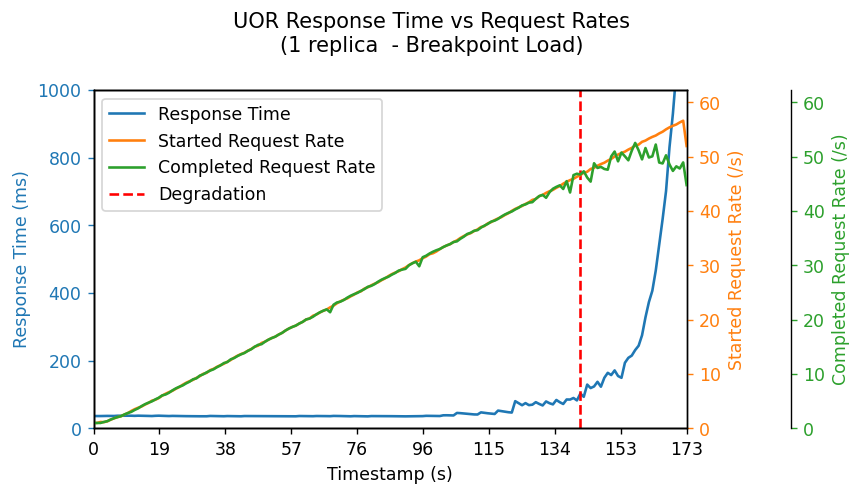
\includegraphics[width=\linewidth]{figures/uor-replica-count-i1-graph-breakpoint.png}
      \caption{1 replica}
    \end{subfigure}%
    \begin{subfigure}{.5\textwidth}
      \centering
      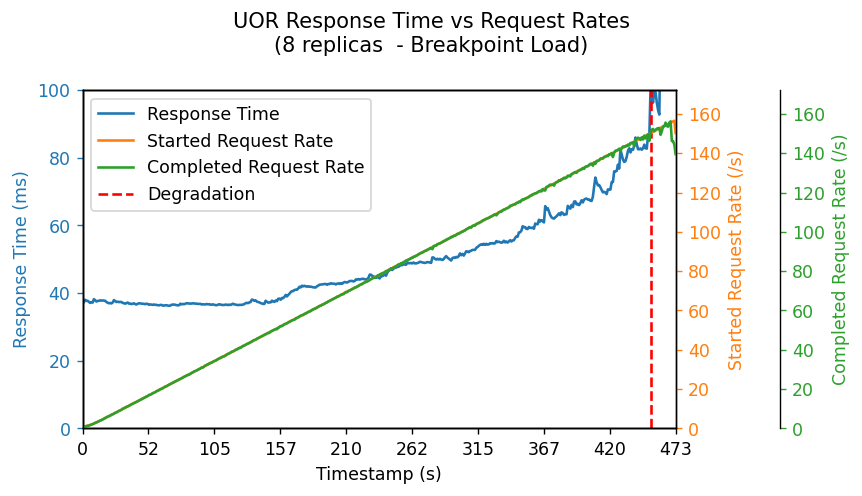
\includegraphics[width=\linewidth]{figures/uor-replica-count-i4-graph-breakpoint.png}
      \caption{8 replicas}
    \end{subfigure}

    \caption{Response time vs. request rate graph (breakpoint load, 1 and 8 replicas)}
    \label{figure:uor-replica-count-graph-breakpoint}
\end{figure}

\begin{figure}[h]
    \centering
    \begin{minipage}{.45\textwidth}
      \centering
      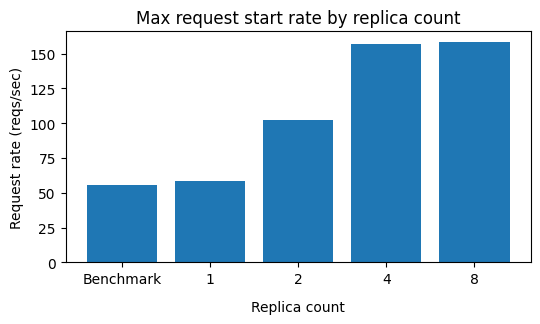
\includegraphics[width=\linewidth]{figures/uor-replica-count-breakpoint-max-reqs.png}

      \caption{Chart of maximum request start rates by replica count}
      \label{figure:uor-replica-count-breakpoint-max-reqs}
    \end{minipage}%
    \hspace{0.09\textwidth} % Adjust the horizontal space here
    \begin{minipage}{.45\textwidth}
      \centering
      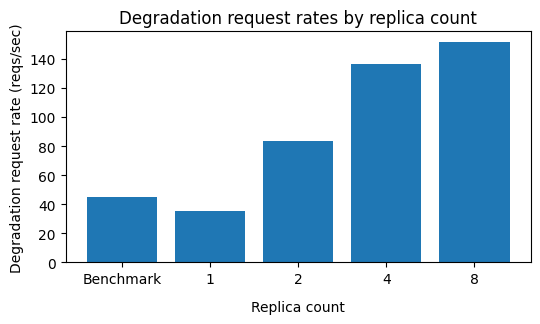
\includegraphics[width=\linewidth]{figures/uor-replica-count-breakpoint-deg-rates.png}

      \caption{Chart of degradation request rates by replica count}
      \label{figure:uor-replica-count-breakpoint-deg-rates}
    \end{minipage}
\end{figure}

In general, a higher number of replicas allows for a higher degradation threshold, though when it comes to the maximum start RPS, the relationship does not appear to be as straightforward. The maximum start RPS only slightly increases from four to eight replicas, which indicates there may be a bottleneck elsewhere in the system preventing a higher maximum.

\subsection{Resource allocation and utilisation}

Results based on a static number of replicas have been showcased, but the effect of dynamic replica auto-scaling on key system metrics is also assessed.

\begin{figure}[H]
    \centering
    \begin{subfigure}{.5\textwidth}
      \centering
      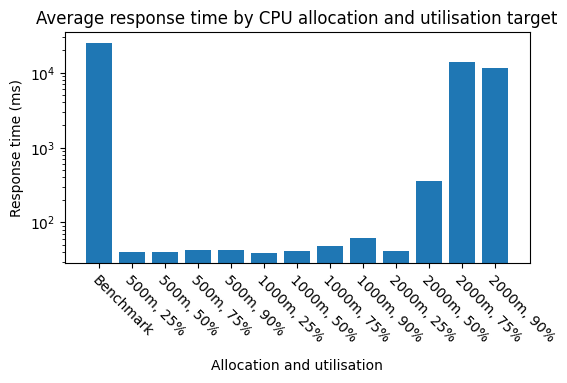
\includegraphics[width=\linewidth]{figures/uor-rau-spike-avg-response-time.png}
      \caption{Logarithmic scale}
    \end{subfigure}%
    \begin{subfigure}{.5\textwidth}
      \centering
      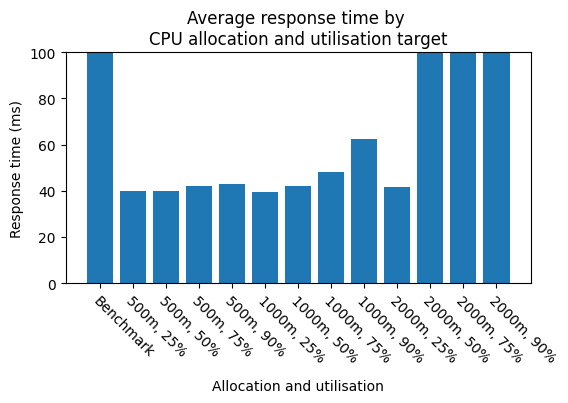
\includegraphics[width=\linewidth]{figures/uor-rau-spike-avg-response-time-2.png}
      \caption{Linear scale}
    \end{subfigure}

    \caption{UOR median response times by CPU allocation and utilisation target (spike load)}
    \label{figure:uor-resource-allocation-rt-comp-spike}
\end{figure}

There are a number of response time patterns that can be observed in Fig. \ref{figure:uor-resource-allocation-rt-comp-spike}. The experiments configured to use 500 millicores of CPU per Django pod have relatively consistent response times, with the lowest median response time being 40.03 milliseconds when the target utilisation is set to 25\%. The lowest response time is, however, claimed by the 1000 millicores and 25\% utilisation combination. Within the 1000 millicore experiments, there is a clear increase in the median response time as the utilisation target is increased, rising to 62.62 milliseconds when set to 90\%.

The 2000 millicore experiments perform poorly on average, save for when the target utilisation is at 25\%. Their median response times range from 355.09 to 11,585 milliseconds. The response time versus request rate graph for the worst performing configuration (2000 millicores with 90\% utilisation target) is seen in Fig. \ref{figure:uor-resource-allocation-rt-graph-i5-i11-spike} (b). It hits the degradation threshold at 46.96 started RPS, and then fails to keep up with further incoming requests. Towards the end of this test, there are missing points for the completed request rate. Since the completed request rate is based on successful requests only, this gap is explained by a period in which all requests failed. In fact, 15.16\% of requests failed with this configuration. When looking at the experiment with 1000 millicores and a 25\% utilisation target, there is a noticeable increase in the response time at the request rate peak (as previously seen in the replica count experiments), but otherwise, no signs of performance degradation are present.

There are three experiments that did not encounter the 100 millisecond degradation threshold: 500 millicores with the 25\% and 50\% targets, and 1000 millicores at 25\%. All other spike load experiments experienced degradation within a range of 16.87 to 49.73 milliseconds.

\begin{figure}[h]
    \centering
    \begin{subfigure}{.5\textwidth}
      \centering
      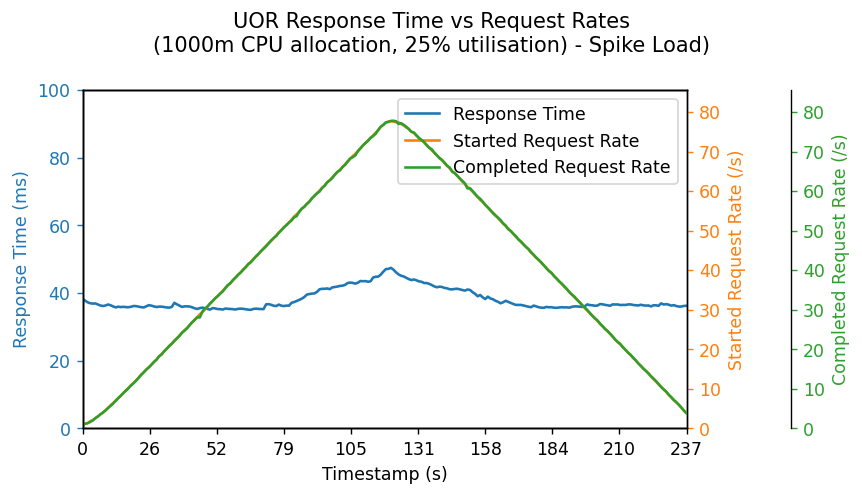
\includegraphics[width=\linewidth]{figures/uor-rau-i5-spike-rt-graph.png}
      \caption{1000m CPU allocation, 25\% target utilisation}
    \end{subfigure}%
    \begin{subfigure}{.5\textwidth}
      \centering
      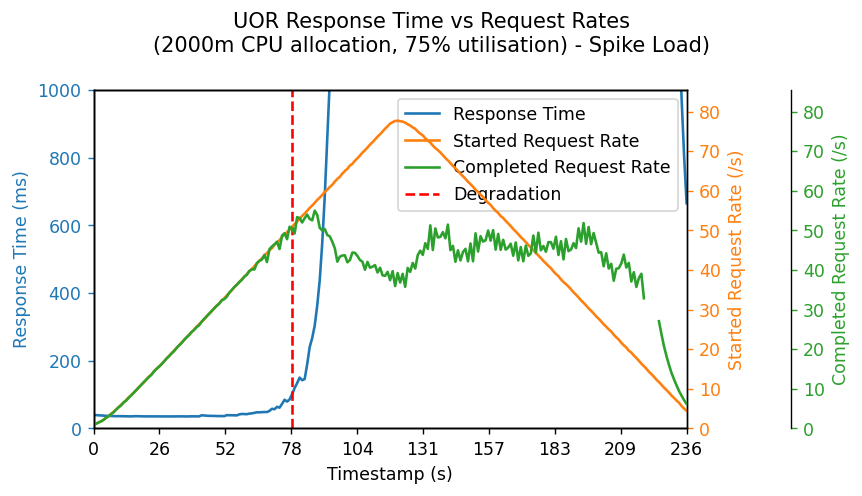
\includegraphics[width=\linewidth]{figures/uor-rau-i11-spike-rt-graph.png}
      \caption{2000m CPU allocation, 75\% target utilisation}
    \end{subfigure}

    \caption{UOR response time vs. request rate graphs (spike load)}
    \label{figure:uor-resource-allocation-rt-graph-i5-i11-spike}
\end{figure}

An observation that can be made (Fig. \ref{figure:uor-resource-allocation-rt-comp-spike}) is that high utilisation targets tend to suffer from poorer response times than low targets, with this being exacerbated when the CPU allocation is simultaneously high. There are several explanations for this. The first is that the Django API has not been configured as a multi-processing application; it does not make use of multiple cores. From this, it is plain to see why a CPU allocation of 2000 millicores results in the worst response time averages, as a utilisation target exceeding 1000 millicores (50\% of 2000 millicores) is unattainable. Secondly, the horizontal pod autoscaler has a reactive rather than predictive nature. As the load on the system increases, previously set utilisation targets are eventually exceeded, and the autoscaler responds by scheduling more replicas in an attempt to meet the target. With higher target utilisation values, individual pods receive higher loads before additional pods spread the overall load further. A higher utilisation target may eventually lead to increased response times, as each API instance attempts to serve more requests at a time, potentially more than can be sustainably handled.

Another clear trend is the negative correlation between the CPU utilisation target and the maximum total requested CPU across all Django API pods. With smaller utilisation targets, the autoscaler schedules pods more frequently in response to increased load, and schedules more pods overall. This can be problematic, as the Kubernetes scheduler uses resource requests to determine whether a node has sufficient capacity to run additional pods, and with provisioning of heavily underutilised resources, nodes may be treated as at capacity, despite low actual resource usage. In this context, as depicted in Fig. \ref{figure:uor-resource-allocation-spike-cpu-allocation}, a 25\% utilisation target with 500 millicores of CPU sees up to 6000 millicores of CPU requested across all Django pods, though only 1500 millicores (1.5 cores) is used in practice based on the target.

\begin{figure}[h]
    \centering
    \begin{minipage}{.45\textwidth}
        \centering
        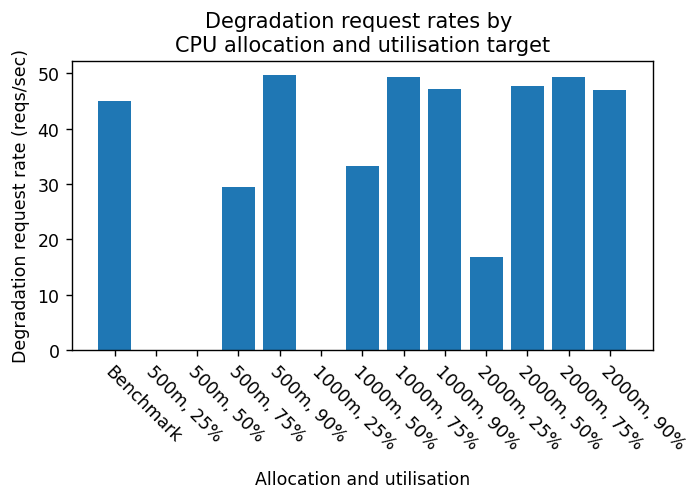
\includegraphics[width=\linewidth]{figures/uor-rau-spike-degradation-reqs.png}
        \caption{Degradation request rates by CPU allocation and utilisation target (spike load)}
        \label{figure:uor-resource-allocation-deg-comp-spike}
    \end{minipage}%
    \hspace{0.05\textwidth} % Adjust the horizontal space here
    \begin{minipage}{.45\textwidth}
      \centering
      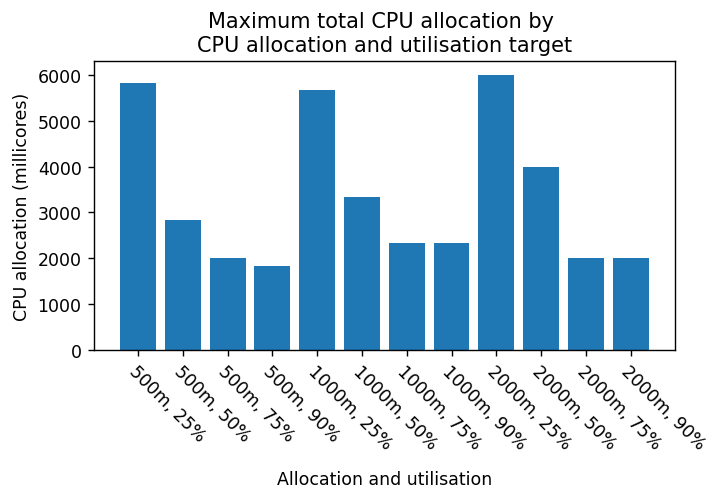
\includegraphics[width=\linewidth]{figures/uor-rau-spike-cpu-allocation.png}

      \caption{CPU allocation by CPU allocation and utilisation target (spike load)}
      \label{figure:uor-resource-allocation-spike-cpu-allocation}
    \end{minipage}
\end{figure}

Within the breakpoint tests, the best performing configuration in terms of the degradation request rate is 500 millicores with a 50\% target (Fig. \ref{figure:uor-resource-allocation-deg-comp-breakpoint}). The response time curve, as shown in Fig. \ref{figure:uor-resource-allocation-rt-graph-i2-i6-breakpoint} (a), shows distinct spikes where the effect of scaling actions can be observed. At approximately 60 started RPS, there is a momentary rise in the response time, which then quickly decreases again. The response time generally increases with the request rate, as seen previously in the replica count tests (Fig. \ref{figure:uor-replica-count-graph-breakpoint}).

\begin{figure}[h]
    \centering
    \begin{subfigure}{.5\textwidth}
      \centering
      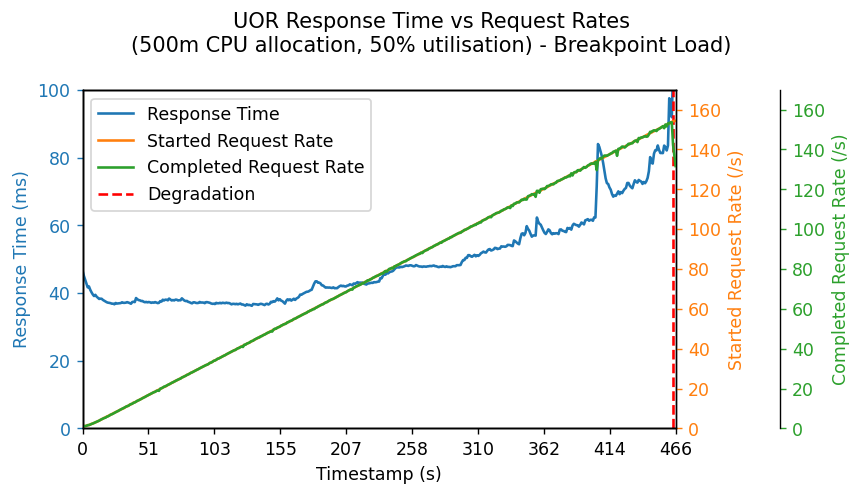
\includegraphics[width=\linewidth]{figures/uor-rau-i2-rt-graph-breakpoint.png}
      \caption{500m CPU allocation, 50\% target utilisation}
    \end{subfigure}%
    \begin{subfigure}{.5\textwidth}
      \centering
      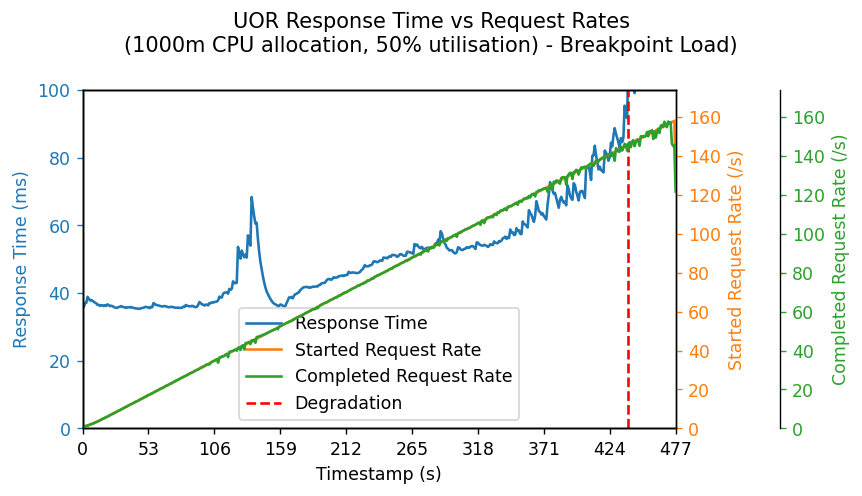
\includegraphics[width=\linewidth]{figures/uor-rau-i6-rt-graph-breakpoint.png}
      \caption{1000m CPU allocation, 50\% target utilisation}
    \end{subfigure}

    \caption{UOR response time vs. request rate graphs (breakpoint load)}
    \label{figure:uor-resource-allocation-rt-graph-i2-i6-breakpoint}
\end{figure}

For 1000 millicores and a 50\% utilisation target, a more pronounced scaling action effect is observed in \ref{figure:uor-resource-allocation-deg-comp-breakpoint} (b). At 45 started RPS, the response time increases by \textasciitilde75\%, and sharply drops. This configuration show signs of greater volatility than the 500 millicores and 50\% target experiment, especially in the latter half of the test. However, another response time spike is seen in \ref{figure:uor-resource-allocation-rt-graph-i2-i6-breakpoint} (a), at \textasciitilde140 started RPS. Despite not crossing the degradation threshold as early as the 1000 millicores experiment, its response time curve does not showcase a perfect load reaction ability of the system. In fact, the 1000 millicores experiment had the highest maximum request start rate (162.33) of all resource allocation experiments, giving evidence that there are various trade offs involved across the configurations.

\begin{figure}[h]
    \centering
    \begin{minipage}{.45\textwidth}
        \centering
        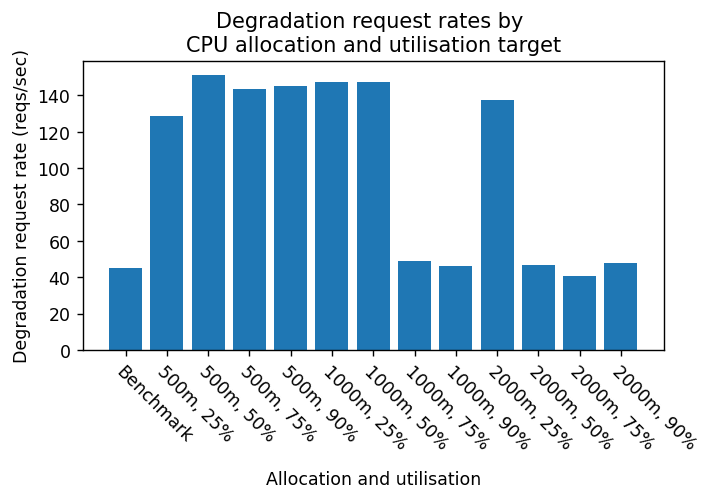
\includegraphics[width=\linewidth]{figures/uor-rau-breakpoint-degradation-reqs.png}
        \caption{UOR degradation request rates by CPU allocation and utilisation target (breakpoint load)}
        \label{figure:uor-resource-allocation-deg-comp-breakpoint}
    \end{minipage}%
    \hspace{0.05\textwidth} % Adjust the horizontal space here
    \begin{minipage}{.45\textwidth}
      \centering
      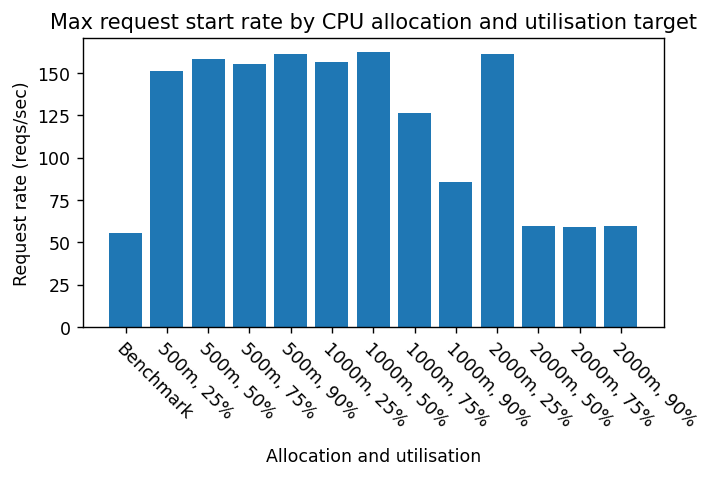
\includegraphics[width=\linewidth]{figures/uor-rau-breakpoint-max-request-rate.png}

      \caption{UOR max request start rates by CPU allocation and utilisation target (breakpoint load)}
      \label{figure:uor-resource-allocation-breakpoint-max-start-rates}
    \end{minipage}
\end{figure}

As before, the 2000 millicore experiments largely performed poorly (Fig. \ref{figure:uor-resource-allocation-deg-comp-breakpoint}). However, in the breakpoint tests, it is observed that the 1000 millicore experiments with 75\% and 90\% targets exceed the degradation threshold early in their respective tests, but do not reach their breakpoints until much later (Fig. \ref{figure:uor-resource-allocation-breakpoint-max-start-rates}). The reason for this pattern is explained by Fig. \ref{figure:uor-resource-allocation-rt-graph-i7-breakpoint}, describing the behaviour of the 1000 millicores, 75\% target experiment. Before reaching the breakpoint, the response time increases by more than 100\% (at \textasciitilde50 started RPS) and drops by the same amount, repeating a similar pattern at \textasciitilde90 started RPS, before rising once more, never returning below 100 milliseconds after this. These repeated spikes show how an inappropriate scaling policy can cause system performance to be very volatile. In this case, the autoscaler takes scaling action too late, allowing for load to increase excessively before scheduling more pods.

\begin{figure}[h]
    \centering
    \begin{minipage}{.45\textwidth}
        \centering
        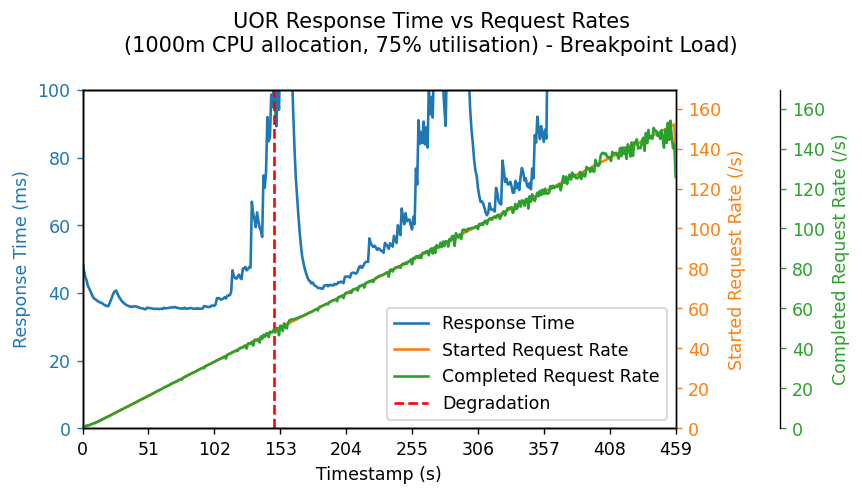
\includegraphics[width=\linewidth]{figures/uor-rau-i7-breakpoint-rt-graph.png}
        \caption{UOR response time vs. request rate graphs (breakpoint load)}
        \label{figure:uor-resource-allocation-rt-graph-i7-breakpoint}
    \end{minipage}%
    \hspace{0.05\textwidth} %
    \begin{minipage}{.45\textwidth}
        \centering
        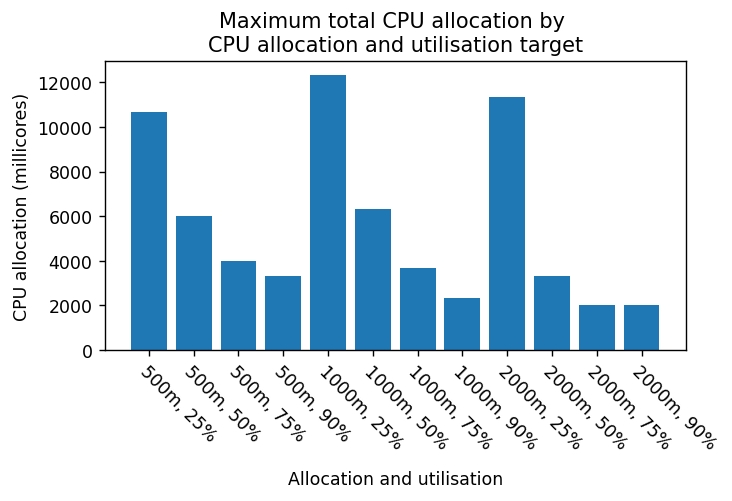
\includegraphics[width=\linewidth]{figures/uor-rau-breakpoint-cpu-allocation.png}
        \caption{UOR CPU allocation by CPU allocation and utilisation target (spike load)}
        \label{figure:uor-resource-allocation-breakpoint-cpu-allocation}
    \end{minipage}
\end{figure}

The breakpoint tests also saw the maximum CPU allocations increase compared with the spike tests (Fig. \ref{figure:uor-resource-allocation-breakpoint-cpu-allocation}), again showing the low target experiments receiving large allocations. The highest allocation comes from the 1000 millicores, 25\% target experiment, at an average maximum of 12,333 millicores. The Kubernetes cluster tested on has 28,000 millicores available, so this allocation is \textasciitilde44\% of the total CPU available.

\section{Flowsheet solving (FS) experiment results}

The following results showcase the performance behaviour of a local deployment of the Ahuora platform versus various scaling configurations for a distributed, Kubernetes-based deployment. In this case, the results are now impacted by two primary software components: the Django API, and the IDAES service.

\subsection{Benchmarks}

\begin{figure}[h]
    \centering
    \begin{minipage}{.47\textwidth}
        \centering
        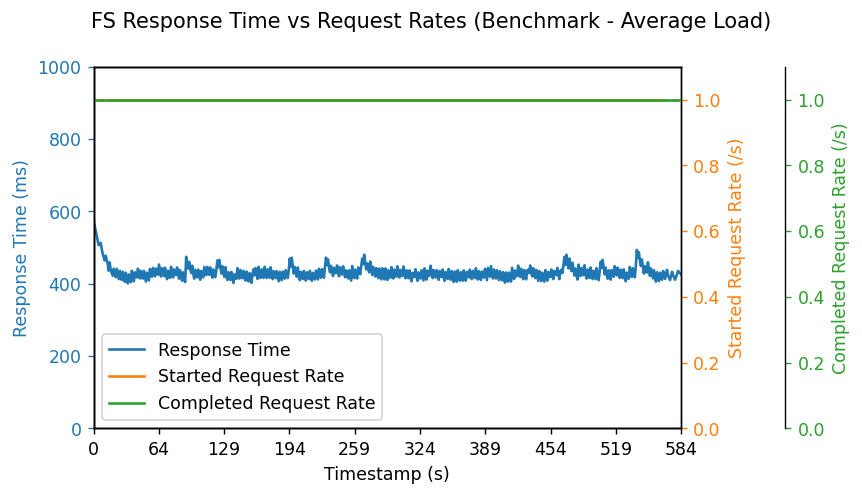
\includegraphics[width=\linewidth]{figures/fs-benchmark-average.png}
        \caption{FS response time vs. request rate graph - average load benchmark}
        \label{figure:fs-benchmark-average}
    \end{minipage}%
    \hspace{0.05\textwidth} % Adjust the horizontal space here
    \begin{minipage}{.47\textwidth}
        \centering
        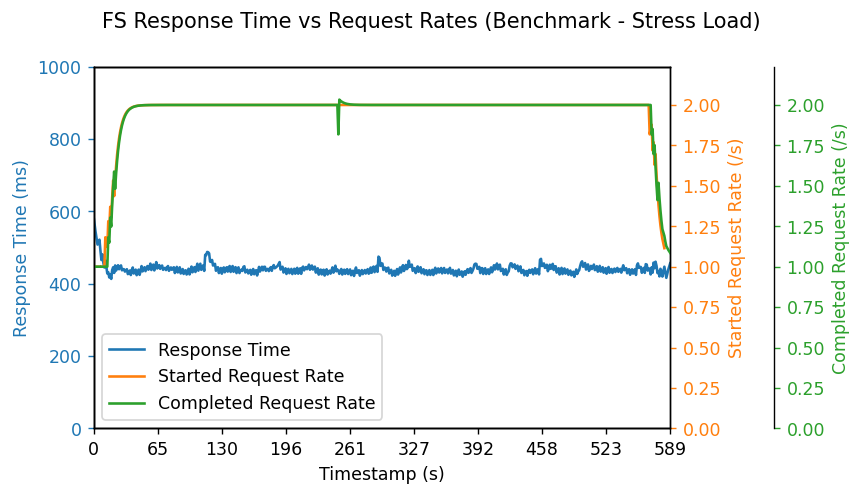
\includegraphics[width=\linewidth]{figures/fs-benchmark-stress.png}
        \caption{FS response time vs. request rate graph - stress load benchmark}
        \label{figure:fs-benchmark-stress}
    \end{minipage}
\end{figure}

\noindent Similarly to the UOR benchmarks, the local deployment has few issues sustaining both the average and stress load profiles (Fig. \ref{figure:fs-benchmark-average} and \ref{figure:fs-benchmark-stress}). However, it can be noted that the median response time of \textasciitilde376 milliseconds under average load is significantly higher than the UOR average load benchmark (\textasciitilde30 milliseconds). The FS API endpoint used does more work than the UOR endpoint (retrieving all data for a flowsheet and performing process simulation), and involves communication between the Django API and the IDAES service. All of this results in the FS endpoint taking longer to fulfil a request on average.

As with the UOR spike test benchmark, the local deployment struggles to complete as many requests as received (Fig. \ref{figure:fs-benchmark-spike}), exceeding the 1000 millisecond threshold after a start request rate of 4.74. The median response time in the spike tests is 4718 milliseconds, more than ten times the average load median response time. Approximately 24\% of spike test requests failed. The breakpoint tests (Fig. \ref{figure:fs-benchmark-breakpoint}) see the degradation request rate being \textasciitilde4.63 RPS, and the start rate reaching no more than 8 RPS.

\begin{figure}[h]
    \centering
    \begin{minipage}{.47\textwidth}
        \centering
        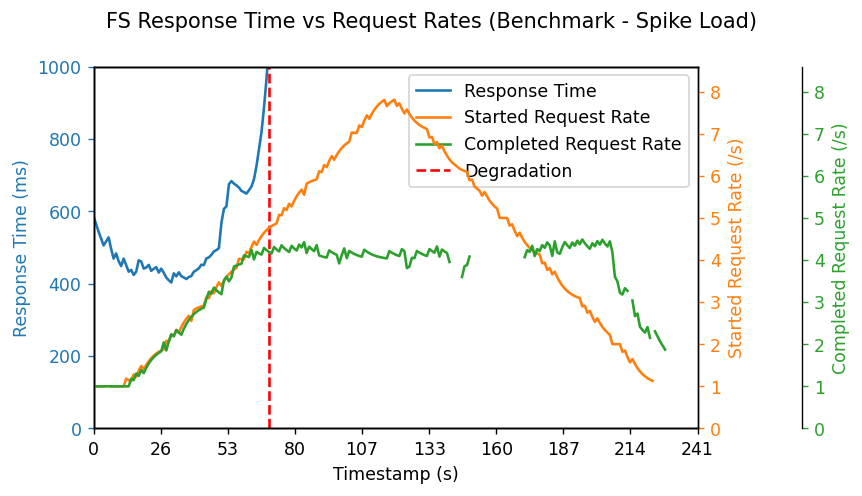
\includegraphics[width=\linewidth]{figures/fs-benchmark-spike.png}
        \caption{FS response time vs. request rate graph - spike load benchmark}
        \label{figure:fs-benchmark-spike}
    \end{minipage}%
    \hspace{0.05\textwidth} % Adjust the horizontal space here
    \begin{minipage}{.47\textwidth}
        \centering
        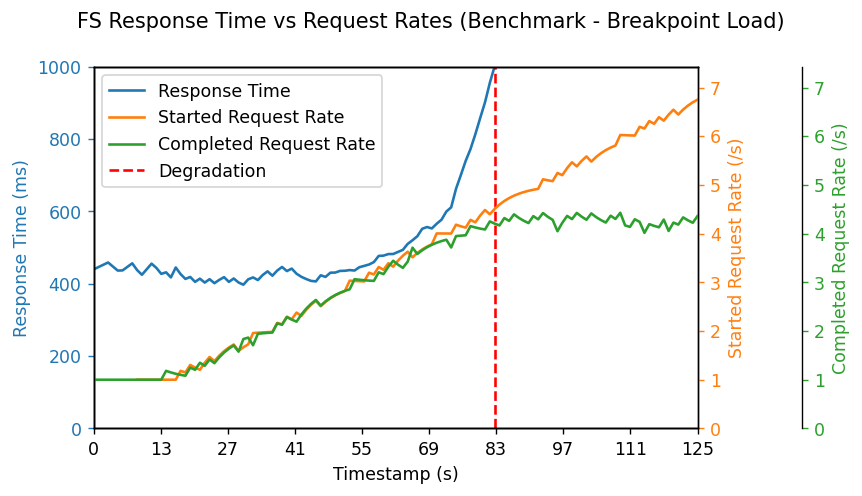
\includegraphics[width=\linewidth]{figures/fs-benchmark-breakpoint.png}
        \caption{FS response time vs. request rate graph - breakpoint load benchmark}
        \label{figure:fs-benchmark-breakpoint}
    \end{minipage}
\end{figure}

\subsection{Replica count}

\begin{figure}[h]
    \centering
    \begin{minipage}{.47\textwidth}
        \centering
        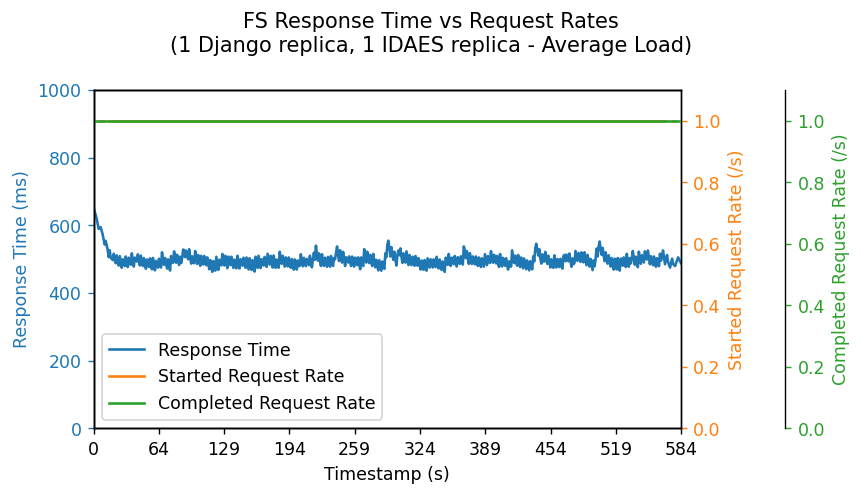
\includegraphics[width=\linewidth]{figures/fs-replica-count-i1-response-graph-average.png}
        \caption{FS response time vs. request rate graph - average load (1 Django replica, 1 IDAES replica)}
        \label{figure:fs-replica-count-i1-average-response-graph}
    \end{minipage}%
    \hspace{0.05\textwidth} % Adjust the horizontal space here
    \begin{minipage}{.47\textwidth}
        \centering
        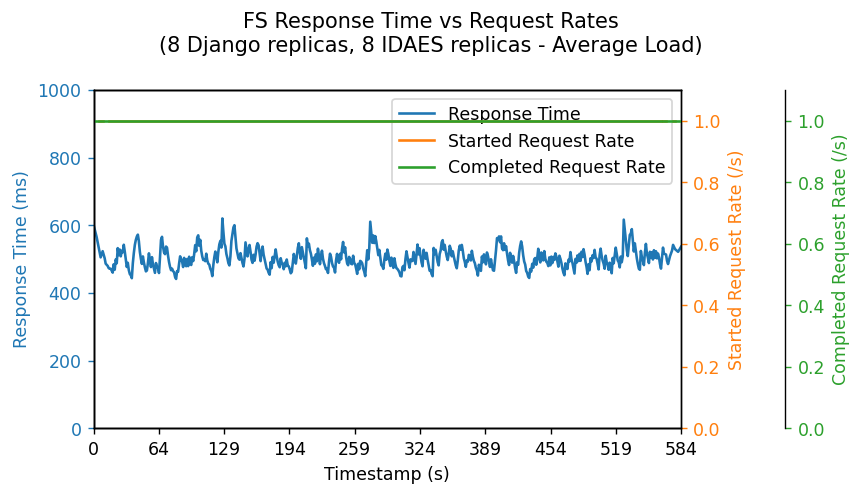
\includegraphics[width=\linewidth]{figures/fs-replica-count-i4-response-graph-average.png}
        \caption{FS response time vs. request rate graph - average load (8 Django replicas, 8 IDAES replicas)}
        \label{figure:fs-replica-count-i4-average-response-graph}
    \end{minipage}
\end{figure}

\noindent An average load applied to the smallest and largest FS replica count configuration behaves similarly to the benchmark (Fig. \ref{figure:fs-replica-count-i1-average-response-graph} and \ref{figure:fs-replica-count-i4-average-response-graph}), with no difference in the ability of the cluster deployment to serve requests compared to the benchmark. As seen in the UOR replica count tests previously, the median response time is between 17\% and 24\% higher (Fig. \ref{figure:fs-response-time-table-average}) with the cluster deployment compared with the benchmark. The potential reasons for this are outlined in \ref{subsection:fs-replica-count}.

\begin{figure}[H]
    \captionsetup{labelformat=empty} % Temporarily disable the default label
    \caption{Table 2: Table of FS median response times by replica count, average load}

    \centering
    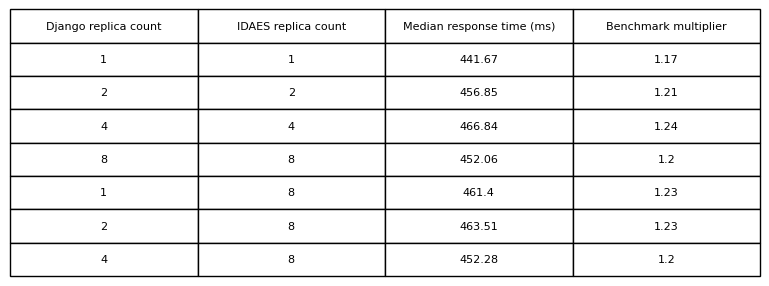
\includegraphics[width=0.8\textwidth]{figures/fs-replica-count-rt-comparison.png}
    \label{figure:fs-response-time-table-average}
\end{figure}

A similar response time pattern to the UOR replica count spike tests is seen in Fig. \ref{figure:fs-replica-count-rt-comp-spike}. A higher number of replicas decreases the median response time, with both the benchmark having an order of magnitude higher response time, and the single replica configuration (both Django and IDAES) between three to four times higher (with 25.44\% of requests having failed). With eight Django and IDAES replicas, the response time is lowest, though the difference is not significant for the spike load profile.

\begin{figure}[H]
    \centering
    \begin{subfigure}{.5\textwidth}
      \centering
      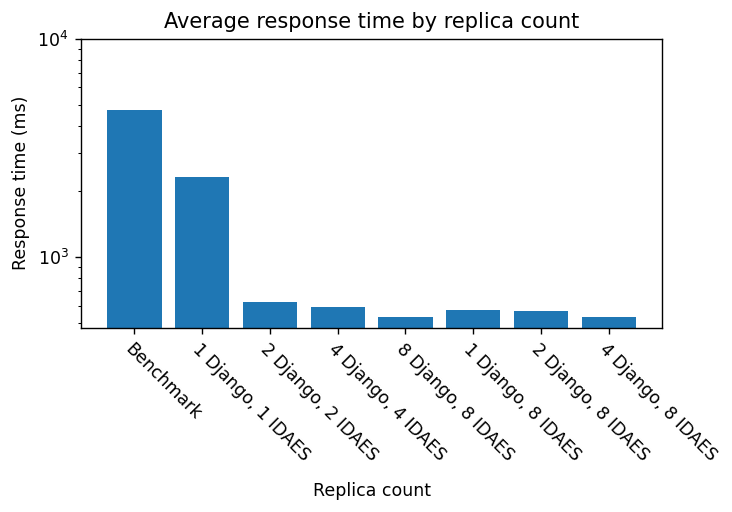
\includegraphics[width=\linewidth]{figures/fs-replica-count-rt-comparison-spike.png}
      \caption{Logarithmic scale}
    \end{subfigure}%
    \begin{subfigure}{.5\textwidth}
      \centering
      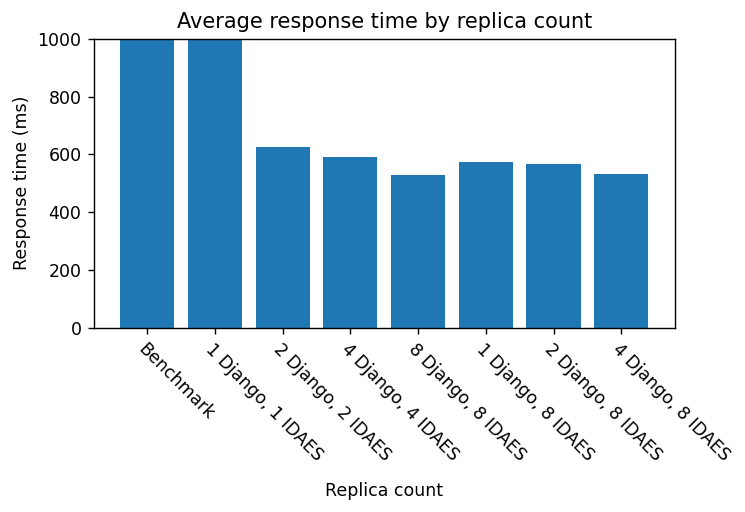
\includegraphics[width=\linewidth]{figures/fs-replica-count-rt-comparison-spike-linear.png}
      \caption{Linear scale}
    \end{subfigure}

    \caption{FS median response times by replica count (spike load)}
    \label{figure:fs-replica-count-rt-comp-spike}
\end{figure}

\begin{figure}[h]
    \centering
    \begin{subfigure}{.5\textwidth}
      \centering
      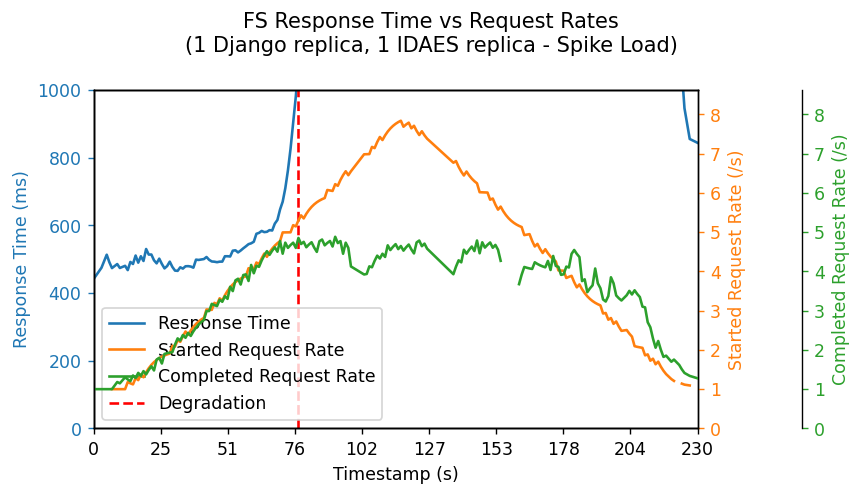
\includegraphics[width=\linewidth]{figures/fs-replica-count-i1-response-graph-spike.png}
      \caption{1 Django and IDAES replica}
    \end{subfigure}%
    \begin{subfigure}{.5\textwidth}
      \centering
      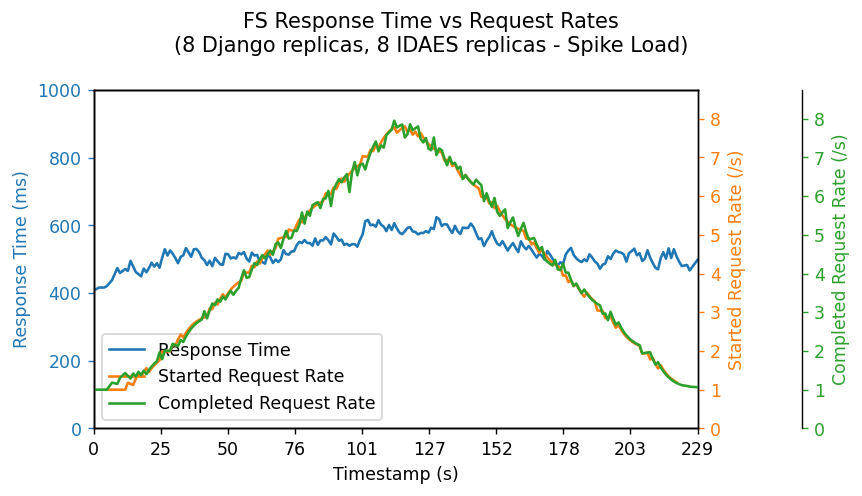
\includegraphics[width=\linewidth]{figures/fs-replica-count-i4-response-graph-spike.png}
      \caption{8 Django and IDAES replicas}
    \end{subfigure}

    \caption{FS response time vs. request rate graph (spike load)}
    \label{figure:fs-replica-count-graph}
\end{figure}

\begin{figure}[h]
    \centering
    \begin{subfigure}{.5\textwidth}
      \centering
      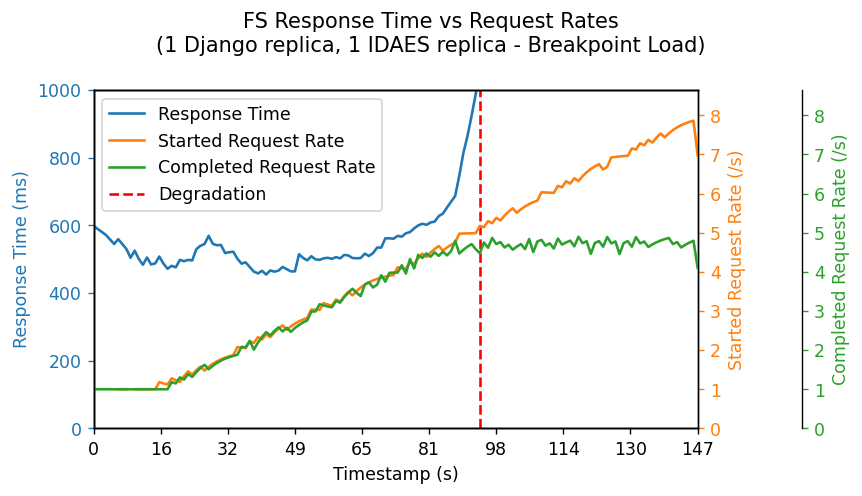
\includegraphics[width=\linewidth]{figures/fs-replica-count-i1-response-graph-breakpoint.png}
      \caption{1 Django and IDAES replica}
    \end{subfigure}%
    \begin{subfigure}{.5\textwidth}
      \centering
      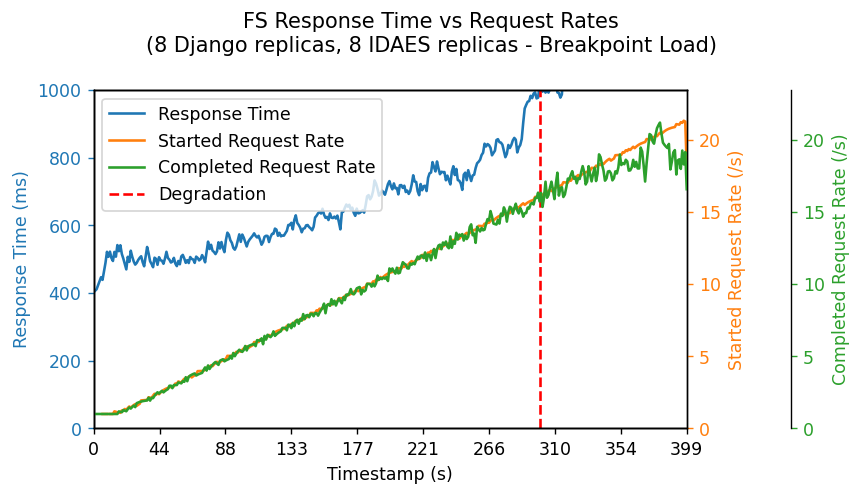
\includegraphics[width=\linewidth]{figures/fs-replica-count-i4-response-graph-breakpoint.png}
      \caption{8 Django and IDAES replicas}
    \end{subfigure}

    \caption{FS response time vs. request rate graph (breakpoint load)}
    \label{figure:fs-replica-count-graph-breakpoint}
\end{figure}

For the single replica configuration, the degradation request rate is 5.17 RPS, which is 9\% higher than that encountered by the benchmark. With the eight replica configuration (Fig. \ref{figure:fs-replica-count-graph} (b)), the system is able to keep the request completion rate consistent with the started request rate, albeit with some volatility. Likewise, a similar degradation request rate of 5.19 RPS is seen in the breakpoint test (Fig. \ref{figure:fs-replica-count-graph-breakpoint}) for the single replica configuration. On the other hand, the degradation request rate with eight replicas is 16.75 RPS. As with the UOR tests, simply increasing the replica count linearly does not likewise linearly increase the degradation request rate or the maximum request start rate reached. Fig. \ref{figure:fs-replica-count-deg-comp-breakpoint} and \ref{figure:fs-replica-count-breakpoint-max-start-rates} both show that the difference between having four or eight Django replicas is not substantial. There is a larger gap between the four and eight IDAES replica scenarios, but even this difference is not more than 37\%.

\begin{figure}[h]
    \centering
    \begin{minipage}{.45\textwidth}
        \centering
        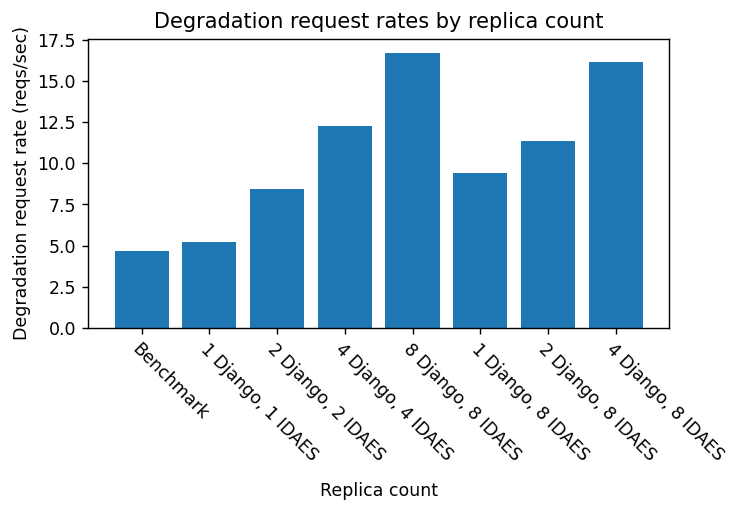
\includegraphics[width=\linewidth]{figures/fs-replica-count-degradation-request-breakpoint.png}
        \caption{FS degradation request rates by replica count (breakpoint load)}
        \label{figure:fs-replica-count-deg-comp-breakpoint}
    \end{minipage}%
    \hspace{0.05\textwidth} % Adjust the horizontal space here
    \begin{minipage}{.45\textwidth}
      \centering
      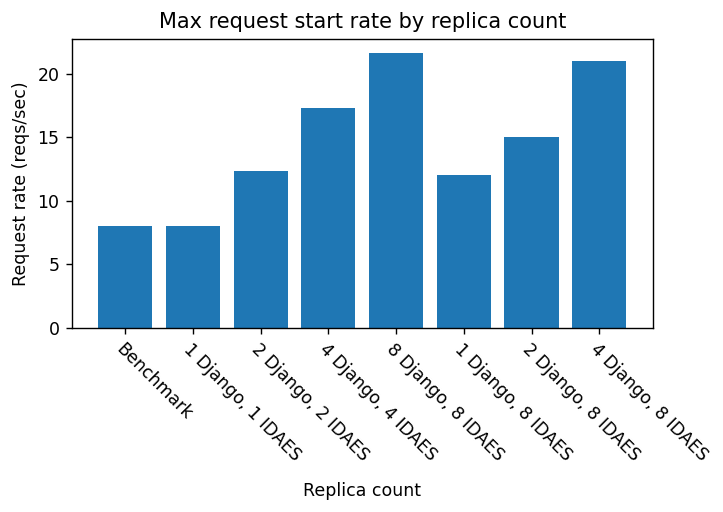
\includegraphics[width=\linewidth]{figures/fs-replica-count-max-requests-breakpoint.png}

      \caption{FS max request start rates by replica count (breakpoint load)}
      \label{figure:fs-replica-count-breakpoint-max-start-rates}
    \end{minipage}
\end{figure}

\subsection{Resource allocation and utilisation}

These resource allocation and utilisation tests show the effect of autoscaling on two logically linked deployments, though the focus is on the scaling of the IDAES service, which has its autoscaling configuration varied between experiments.

\begin{figure}[H]
    \centering
    \begin{subfigure}{.5\textwidth}
      \centering
      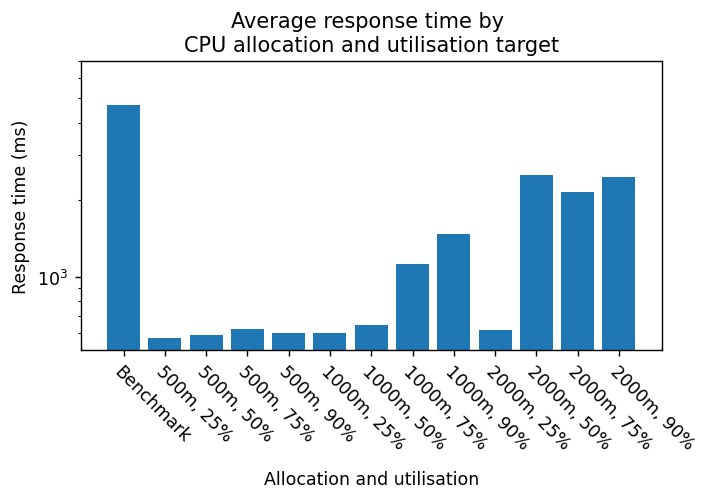
\includegraphics[width=\linewidth]{figures/fs-rau-median-response-spike-log.png}
      \caption{Logarithmic scale}
    \end{subfigure}%
    \begin{subfigure}{.5\textwidth}
      \centering
      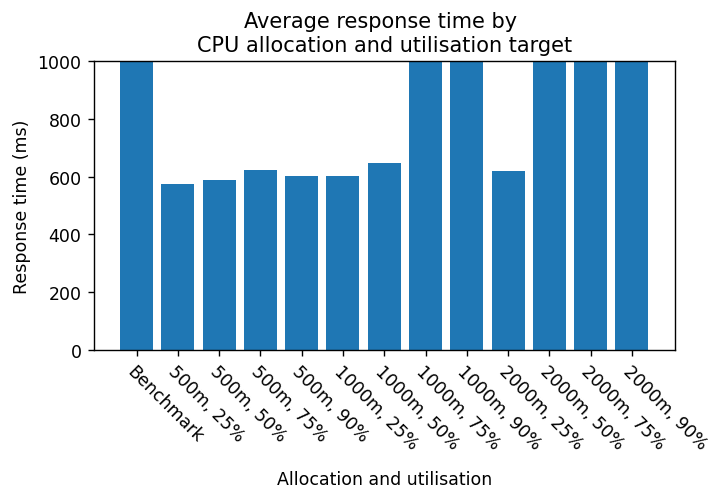
\includegraphics[width=\linewidth]{figures/fs-rau-median-response-spike-linear.png}
      \caption{Linear scale}
    \end{subfigure}

    \caption{FS median response times by CPU allocation and utilisation target (spike load)}
    \label{figure:fs-resource-allocation-rt-comp-spike}
\end{figure}

As Fig. \ref{figure:fs-resource-allocation-rt-comp-spike} shows, all of the 500 millicores allocation configurations had relatively consistent median response times under the spike load tests, while the utilisation target seems to play a much more important role for the 1000 millicores allocations. The 75\% and 90\% targets experienced significantly higher median response times when 1000 millicores was allocated. As has been seen numerous times previously, all but the 25\% target of the 2000 millicores set have extremely poor response time performance, though not as high as the benchmark. The lowest response time is achieved by the 500 millicore, 25\% target configuration. However, the only configuration that does not suffer from breaches of the degradation threshold is a 500 millicores and 90\% target (Fig. \ref{figure:fs-resource-allocation-deg-comp-spike}), with the rest ranging from 4 to 8 degradation RPS levels. Fig. \ref{figure:fs-resource-allocation-rt-graph-i4-i6-spike} (a)presents the performance of this configuration over the course of a test: the response time (somewhat erratically) increases with the request rate, but remains below 1000 milliseconds, before stabilising downwards as the request rate decreases. Fig. \ref{figure:fs-resource-allocation-rt-graph-i4-i6-spike} (b) displays instead the slow system reactivity with a 1000 millicores allocation and 50\% target. The response time spikes, and before the peak request rate, it returns to a new baseline, before increasing again along with the request rate.

\begin{figure}[h]
    \centering
    \begin{subfigure}{.5\textwidth}
      \centering
      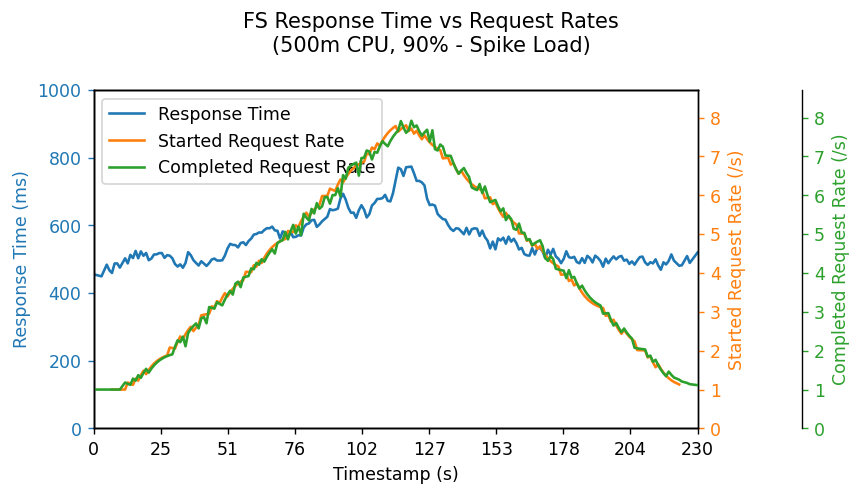
\includegraphics[width=\linewidth]{figures/fs-rau-i4-response-curve-spike.png}
      \caption{500m CPU allocation, 90\% target utilisation}
    \end{subfigure}%
    \begin{subfigure}{.5\textwidth}
      \centering
      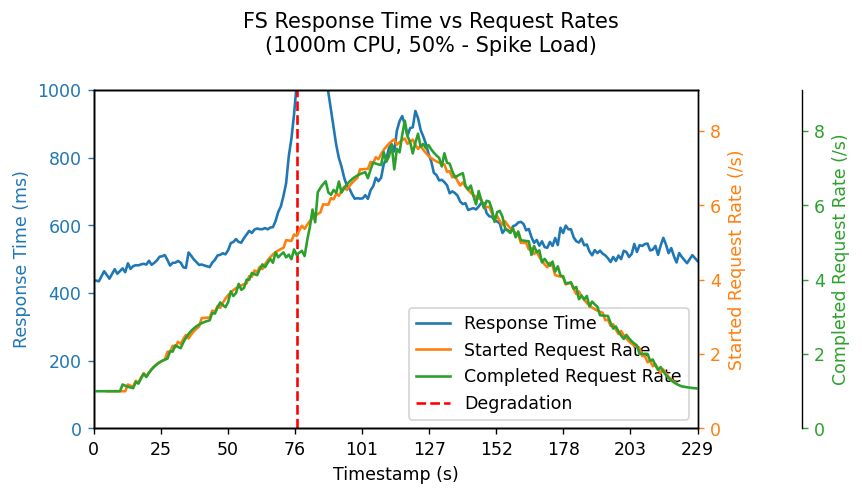
\includegraphics[width=\linewidth]{figures/fs-rau-i6-response-curve-spike.png}
      \caption{1000m CPU allocation, 50\% target utilisation}
    \end{subfigure}

    \caption{FS response time vs. request rate graphs (spike load)}
    \label{figure:fs-resource-allocation-rt-graph-i4-i6-spike}
\end{figure}

\noindent Fig. \ref{figure:fs-resource-allocation-spike-cpu-allocation} shows a pattern that has presented itself in the UOR resource allocation and utilisation tests: low utilisation targets result in high total CPU allocation. Whether the subject workload is the Django API or the IDAES service, this pattern seems to remain true.

\begin{figure}[H]
    \centering
    \begin{minipage}{.45\textwidth}
        \centering
        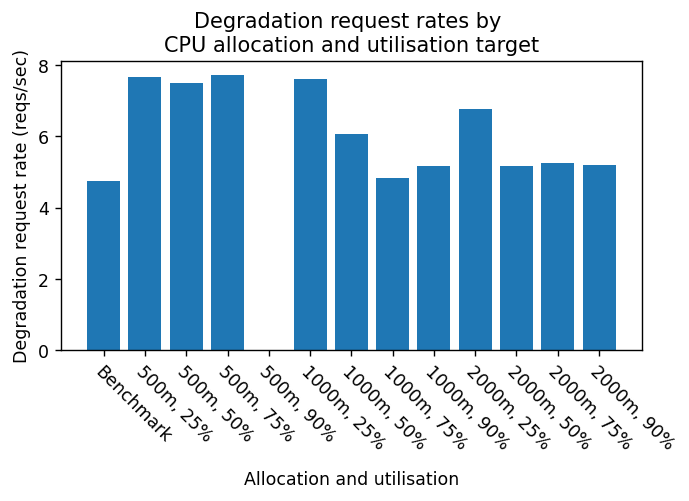
\includegraphics[width=\linewidth]{figures/fs-rau-spike-degradation-rates.png}
        \caption{FS degradation request rates by CPU allocation and utilisation target (spike load)}
        \label{figure:fs-resource-allocation-deg-comp-spike}
    \end{minipage}%
    \hspace{0.05\textwidth} % Adjust the horizontal space here
    \begin{minipage}{.45\textwidth}
      \centering
      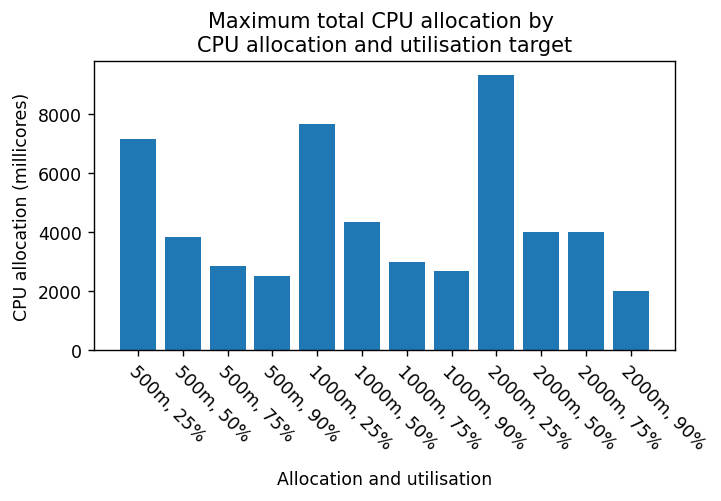
\includegraphics[width=\linewidth]{figures/fs-rau-cpu-allocation-spike.png}

      \caption{FS CPU allocation by CPU allocation and utilisation target (spike load)}
      \label{figure:fs-resource-allocation-spike-cpu-allocation}
    \end{minipage}
\end{figure}

\begin{figure}[h]
    \centering
    \begin{subfigure}{.5\textwidth}
      \centering
      \includegraphics[width=\linewidth]{figures/fs-rau-i5-response-curve-breakpoint.png}
      \caption{1000m CPU allocation, 25\% target utilisation}
    \end{subfigure}%
    \begin{subfigure}{.5\textwidth}
      \centering
      \includegraphics[width=\linewidth]{figures/fs-rau-i7-response-curve-breakpoint.png}
      \caption{1000m CPU allocation, 75\% target utilisation}
    \end{subfigure}

    \caption{FS response time vs. request rate graphs (breakpoint load)}
    \label{figure:fs-resource-allocation-rt-graph-i5-i7-breakpoint}
\end{figure}

\noindent In the breakpoint tests, the best configuration with respect to the degradation request rate is that with 1000 millicores allocated and a 25\% target, reaching 16.43 RPS (\textasciitilde3.5 times the benchmark) before exceeding the 1000 millisecond threshold (Fig. \ref{figure:fs-resource-allocation-deg-comp-breakpoint}). It can be noted that, despite this, the response time is still quite volatile, and there is evidence of slow scaling actions at several points in the test (Fig. \ref{figure:fs-resource-allocation-rt-graph-i5-i7-breakpoint}). Along with this, the total CPU allocation across the cluster by this configuration was 22,000 millicores (Fig. \ref{figure:fs-rau-cpu-allocation-breakpoint}), or 22 cores, the second-highest allocation of all configurations. This value constitutes \textasciitilde78.6\% of all available CPU on the cluster, which is likely to cause significant scheduling issues for other deployments.

\begin{figure}[H]
    \centering
    \begin{minipage}{.45\textwidth}
        \centering
        \includegraphics[width=\linewidth]{figures/fs-rau-breakpoint-degradation-rates.png}
        \caption{FS degradation request rates by CPU allocation and utilisation target (breakpoint load)}
        \label{figure:fs-resource-allocation-deg-comp-breakpoint}
    \end{minipage}%
    \hspace{0.05\textwidth} % Adjust the horizontal space here
    \begin{minipage}{.45\textwidth}
      \centering
      \includegraphics[width=\linewidth]{figures/fs-rau-max-request-start-breakpoint.png}

      \caption{FS max request start rates by CPU allocation and utilisation target (breakpoint load)}
      \label{figure:fs-resource-allocation-breakpoint-max-start-rates}
    \end{minipage}
\end{figure}

\begin{figure}[H]
    \centering
    \includegraphics[width=0.6\textwidth]{figures/fs-rau-cpu-allocation-breakpoint.png}
    \caption{FS CPU allocation by CPU allocation and utilisation target (breakpoint load)}
    \label{figure:fs-rau-cpu-allocation-breakpoint}
\end{figure}

\noindent Across both the UOR (unit operation retrieval) and FS (flowsheet solving) experiments, a selection of scaling configurations allow the number of requests processed in a stable fashion to increase by three to four times, allowing more analysis to be conducted, and more users to access the platform. However, as indicated by the diminishing returns when increasing the number of replicas (for either the Django API or the IDAES service), there is evidence that bottlenecks exist in the system (a component is slowing the system down), which will need further investigation.

\section{Impacts}

With the successful migration of the Ahuora Digital Twin Platform to a distributed Kubernetes cluster, the platform is now able to take advantage of additional processing power, with no need to invest in individually powerful machines to perform efficient process modelling, optimisation and analysis at scale. Additionally, by making use of a cloud-native environment, expanding the platform's capabilities becomes more straightforward. New internal software services can be easily integrated into the existing system architecture, and the expansive world of community cloud-native software can likewise serve to extend platform functionality.

Having performed empirical performance testing and analysis, the produced data can be used to inform further optimisation of the deployed software, in particular the Django API and IDAES service, which are core pieces of the Ahuora platform. By appropriately setting resource allocation requests and utilisation targets, the platform will be able to handle variable system load while avoiding unnecessary overprovisioning of cluster resources, which can be allocated to other deployed software.

\section{Threats to validity}

There are some elements of this work that could impact the legitimacy of the obtained results, or at the very least, their usefulness in practice. First, the metrics collected at one-minute intervals from the cluster during performance testing make it difficult to perform fine-grained analysis on how all parts of the internal system are behaving. Client-side performance data, from the perspective of the k6 test client, is plentiful, but this is not the case with system metrics. Such a long interval means that very short-term behaviour (like pod scaling actions) may be missing, or otherwise inaccurately captured.

Another potential cause for concern is the limited scaling configuration parameter space explored. Because of the limited time available to conduct extensive testing, some parameter combinations could not be explored in full. For example, with the flowsheet solving resource allocation and utilisation tests, the scaling settings for the IDAES service were varied, but the Django API settings were fixed, despite the API being a core part of the solving pipeline. It is highly likely that a restructuring of the solving pipeline will prevent this from being an issue in future.